%%%%%%%%%%%%%%%%%%%%%%%%%%%%%%%%%%%%%%%%%%%%%%%%%%%%
% This will help you in writing your homebook
% Remember that the character % is a comment in latex
%
% chapter 1
\chapter{Introduction}
\label{chap1}

\section{Motivation}
A lot of EDA tools used a heuristic approaches to solve synthesis for electronic circuits. In high level synthesis (HLS) there could be two types of constrained: area or time. Exact algorithms are not use to solve those kinds of problems because solutions will occur after a lot of time, even years. In this project the main purpose is to exploit the parallelism of the GPU to create all the possible set of combination of resources, that satisfy area constrain, and through the usage of a list scheduling algorithm evaluate which is the fastest among all.

To evaluate all the benefits of GPU algorithm version a CPU one has been written. The basic concept is the same but in the latter a the classical sequential approach has been used.

\section{Terms clarification}

Before to move on a little refresh about general topic of this project is mandatory.

Synthesis is the process that generate the circuit netlist of a certain circuit model, given a set of library and a target device. High level synthesis (HLS), also known as behavioral synthesis and algorithmic synthesis, is a design process in which a high level functional description of a design is automatically compiled into a RTL implementation that meets certain user specified design constraints. 

Topically HLS is divided in three main phase:

\begin{itemize}
    \item Allocation, choice of how many resources will be used;
    \item Scheduling, of the processes on the set of selected resources;
    \item Binding of operations to resources.
\end{itemize}{}

Simultaneous solution of these three problems would lead to better results (closer to the Pareto-optimal set), but it is typically too complex.
A Pareto point is a solution that is better than the other under certain aspect and is not dominated by any other.

\subsection{List scheduling}
\label{list_scheduling}

List scheduling is a greedy algorithm that takes as inputs a list of jobs that should be executed on a set of resources, that is also given. The list is ordered according a priority criteria, that could be not always the same. The algorithm repeatedly executes the following steps until a valid schedule is obtained:
\begin{itemize}
    \item Take the first job in the list (the one with the highest priority).
    \item Find a resources that is available for executing this job.
    \item If a resources is found, schedule this job on it, otherwise (no suitable machine is available), select the next job in the list.
    \item Repeat until resources are not more available or there are not node to schedule.
\end{itemize}

To obtain a valid schedule all nodes have to been scheduled in a finite time respected the resources number constraints.

\subsection{Example}
Let's try to synthesis the following function $F = a*b + a*c$, that is represented by the DFG in figure \ref*{fig:DFG}. It's important to note that each node of the DFG is binary, receive at most two inputs, and that each node will be assign to a specific resources in a given instant of time.

\begin{figure}[h]
\centering
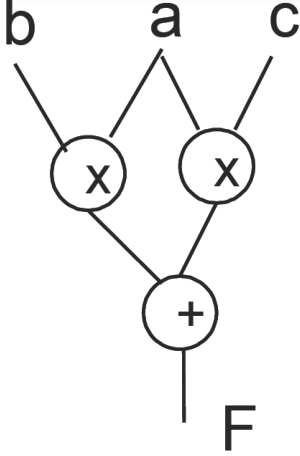
\includegraphics[height=5cm]{chapters/figures/dfg.png}
\caption{DFG of $F = a*b + a*c$}
\label{fig:DFG}
\end{figure}

Two possible schedules could be picked, like shows in figure \ref{fig:DFG_schedules}. Both are Pareto-optimal but in the left one just two resources have been used (one adder and one multiplier) while in the right one is present a further multiplier. Of curse the latter has littler latency.
 
\begin{figure}[h]
\centering
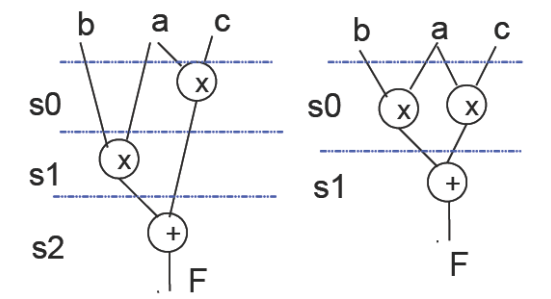
\includegraphics[height=5cm]{chapters/figures/dfg_scheduled.png}
\caption{On the left there is a bigger latency but less resources are used, while on the right a littler latency occur but more resource are used.}
\label{fig:DFG_schedules}
\end{figure}

The purpose of this project is to select the set of resources that allows to have the lowest latency and that respect a certain value of area constraint.
In this case let's suppose that each resources has an unitary value of area and the limit is 2,  the first schedules will be the one chosen.

The following schedules is then convert in hardware, like shows in figure \ref{fig:HW_schedules}.

\begin{figure}[h]
\centering
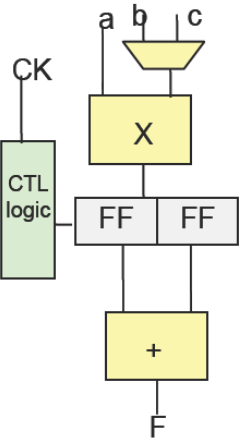
\includegraphics[height=6cm]{chapters/figures/HW_scheduling.png}
\caption{Hardware implementation}
\label{fig:HW_schedules}
\end{figure}

\section{How to proceed}

The synthesis tools used to schedule DFG through the usage of efficient heuristic solutions that find optimal solutions because those approaches are not exhaustive and don't use exact scheduling algorithm (like ILP). 

The purpose of this project is to explore all the set of resources combinations and, based on a list scheduling algorithm, choose which one retrieve the smallest latency. In order to do that GPU is exploited to create all those combinations in parallel and for each calculate the schedule time using the same criteria.

As first attempt a sequential version, runnable on CPU, has been written and different versions for GPU, in order too see which one will be the fastest.

All the available DFGs used for test have been taken from another course and for this project purpose the format has been a little modify, through a python algorithm, to have a faster computation in cuda language. The original one are available and usable to retrieve a visual interpretation of operations.








